%%%%%%%%%%%%%%%%%%%%%%%%%%%%%%%%%%%%%%%%%%%%%%%%%%%%%%%%%%%%%%%
%
% Welcome to Overleaf --- just edit your LaTeX on the left,
% and we'll compile it for you on the right. If you open the
% 'Share' menu, you can invite other users to edit at the same
% time. See www.overleaf.com/learn for more info. Enjoy!
%
%%%%%%%%%%%%%%%%%%%%%%%%%%%%%%%%%%%%%%%%%%%%%%%%%%%%%%%%%%%%%%%
\documentclass[17pt, a0paper, landscape,  margin=0mm, innermargin=10mm, blockverticalspace=3mm, colspace=3mm, subcolspace=3mm]{tikzposter}
\usepackage{graphicx}
\usepackage{authblk}
\usepackage{color}
\usepackage[all]{xy}

\usetheme{board}

%% Elena's favorite green (thanks, Fernando!)
\definecolor{ForestGreen}{RGB}{34,139,34}
\definecolor{BlueViolet}{RGB}{138,43,226}
\definecolor{Coquelicot}{RGB}{255, 56, 0}
\definecolor{Teal}{RGB}{2,132,130}
%Uncomment this if you want to show work-in-progress comments
\newcommand{\comment}[1]{{\bf \tt  {#1}}}
% Uncomment this if you don't want to show comments
%\newcommand{\comment}[1]{}
% for color names see https://www.overleaf.com/learn/latex/Using_colors_in_LaTeX
\newcommand{\emcomment}[1]{\textcolor{ForestGreen}{\comment{Elena: {#1}}}}
\newcommand{\todo}[1]{\textcolor{blue}{\comment{To Do: {#1}}}}
\newcommand{\tkcomment}[1]{\textcolor{Teal}{\comment{Tristan: {#1}}}}
\newcommand{\jscomment}[1]{\textcolor{olive}{\comment{Jaydon: {#1}}}}
\newcommand{\jwcomment}[1]{\textcolor{violet}{\comment{John: {#1}}}}

\title{Breaking Down Terminology of Clojure Error Messages for Beginner Programmers.}
\author[1]{John Walbran}
\author[1]{Jaydon Stanislowski}
\author[1]{Tristan Kalvoda}
\author[1]{Elena Machkasova (adviser)}
\date{\today}
\affil[1]{Division of Science and Mathematics, University of Minnesota, Morris}
\usetheme{Envelope}
\usecolorstyle{Australia}

\begin{document}

\makeatletter
\def\maketitle{\AB@maketitle}
\makeatother

\maketitle

\block{Abstract}{
The Clojure programming language has educational potential for beginner programmers due to its clean, simple syntax and its strong focus on functional programming, an important aspect of CSci education. However, one weakness of Clojure lies in its error messages, which are messages that programmers receive when a program goes wrong. The terminology and shorthands used to convey necessary information for understanding the error are often confusing to novices. The issue is exacerbated by the fact that the error messages are phrased in terms of the underlying programming language – Java – which beginner programmers may typically be unfamiliar with. A research group at UMN Morris is developing a tool, called Babel, that replaces the language's default error messages with less jargon-heavy forms. This year, we started utilizing a graphical interface for viewing Clojure data to highlight the important details and terminology via context-based formatting choices, designed to make it possible for users to easily explore the reasons for the error and get access to relevant resources. We present our work-in-progress design of displaying error messages and discuss its potential benefits for new learners. 
%\emcomment{Needs to be shortened and changed to match this year's work}
}
\begin{columns}
\column{0.3}
        \block{Overview of Functional Programming and Clojure}{
%\tkcomment{Tristan's section}
    \begin{itemize}
%	\item \emcomment{Includes reasons to teach FP to beginners}
	\item Functional programming has a rich history of being introduced early in programming education [4].
	\item It emphasizes breaking problems into smaller, manageable, easy-to-combine pieces.
%promotes a more declarative programming style. Which is where you tell it what you want to happen rather than giving it a list of steps to follow.
	\item It builds a strong foundation for students in subjects like recursion, higher-order functions, immutable data, and problem decomposition.
    \item Clojure is a functional language
%Lisp-based language 
that encourages these principles and is a great tool for introducing students to functional programming.
    \item It has a simple, minimal syntax with prefix notation in statements and statements are surrounded by parentheses: \texttt{(+ 2 3)} is the way to write $2 + 3$.
    \item It uses an interactive Read-Evaluate-Print-Loop (REPL) environment: the user types some code, the system evaluates it and prints the answer.
    \end{itemize}
}

 \block{Clojure Error Messages}{
%\tkcomment{Tristan's section}
    \begin{itemize}
    \item Error messages are understandable to experienced developers, but have terminology that does not make sense to beginner programmers.
    \item Clojure code is compiled into a more common language, Java. It is a more complex language whose data types and features are not known to beginner programmers. 
   \item By the time Clojure code is executed, it is Java code, so Clojure errors appear as Java errors.
%\emcomment{The target audience doesn't know the difference.}
    \item Error messages include Java error types and a Java-phrased cause, as well as a Clojure location.
    \end{itemize}
}

\block{Our Project, Babel}{
    \begin{itemize}
        \item One focus of our research is development of a tool called Babel to modify Clojure error messages.
        \item Many error messages are directly replaced in the REPL with simplified, beginner-friendly versions.
        \item Errors on function calls provide more detailed information about expected arguments: their types, number, etc.
        \item Babel categorizes error data via dictionary lookup and specifications on Clojure function requirements to achieve this. 
        \item We developed and designed these specifications to capture as much information for the end user as possible, which is absent in default Clojure messages.
    \end{itemize}
}

\block{Goals for This Year.}{
    \begin{itemize}
        \item Presently, we are working with a tool called Morse to provide an interactive user interface for Babel.
        \item Morse is a data visualization tool designed for professional development and debugging [2].
        \item In the past, we succeeded in integrating Morse with Babel. Now, we are modifying information flow between the tools to provide Morse with more capabilities.
        \item We are aiming to have Morse stylize text based on good design practices for error messages [3].
    \end{itemize}
    }

\column{0.4}
    \block{Examples}{
%\jwcomment{John's section.}
%\emcomment{(even? "two"), (even? 2 3)}
    Correct call: \\
    \texttt{user=>(even? 2)} \\
    \texttt{true} \\

    Default Clojure: \\
    \texttt{user=>(even? "two")} \\
    \texttt{Execution error (IllegalArgumentException) at user/eval2044 (REPL:1).}\\
    \texttt{Argument must be an integer: two}


    \texttt{user=>(even? 2 3)} \\
    \texttt{Execution error (ArityException) at user/eval2046 (REPL:1).} \\ 
     \texttt{Wrong number of args (2) passed to: clojure.core/even?} \\

    Babel (in REPL): \\
    \texttt{user=>(even? "two")}\\
    \texttt{The first argument of (even? "two") was expected to be a number but is a string "two" instead.}\\
    \texttt{In Clojure interactive session on line 1.}


    \texttt{user=>(even? 2 3)} \\
    \texttt{Wrong number of arguments in (even? 2 3): the function even? expects one argument but was given two arguments.}\\
    \texttt{In Clojure interactive session on line 1.} \\

    Babel (with Morse) Pop-up: \\
    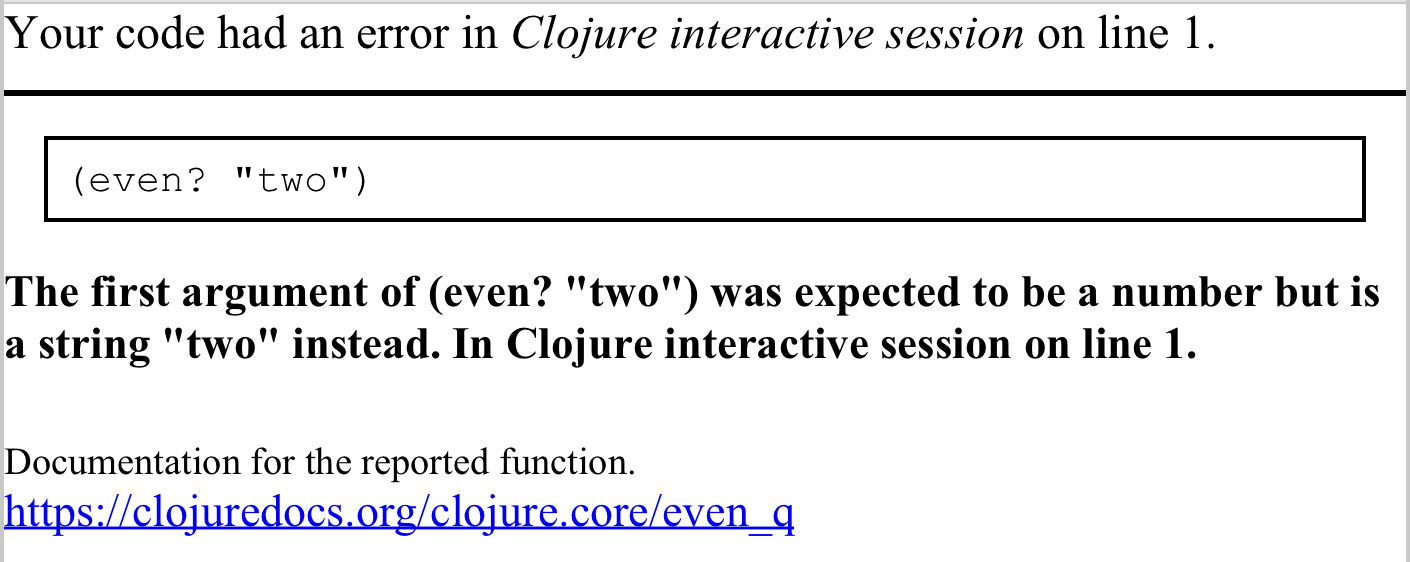
\includegraphics[width=\linewidth]{figures/ErrorViewer1Cropped.png}
    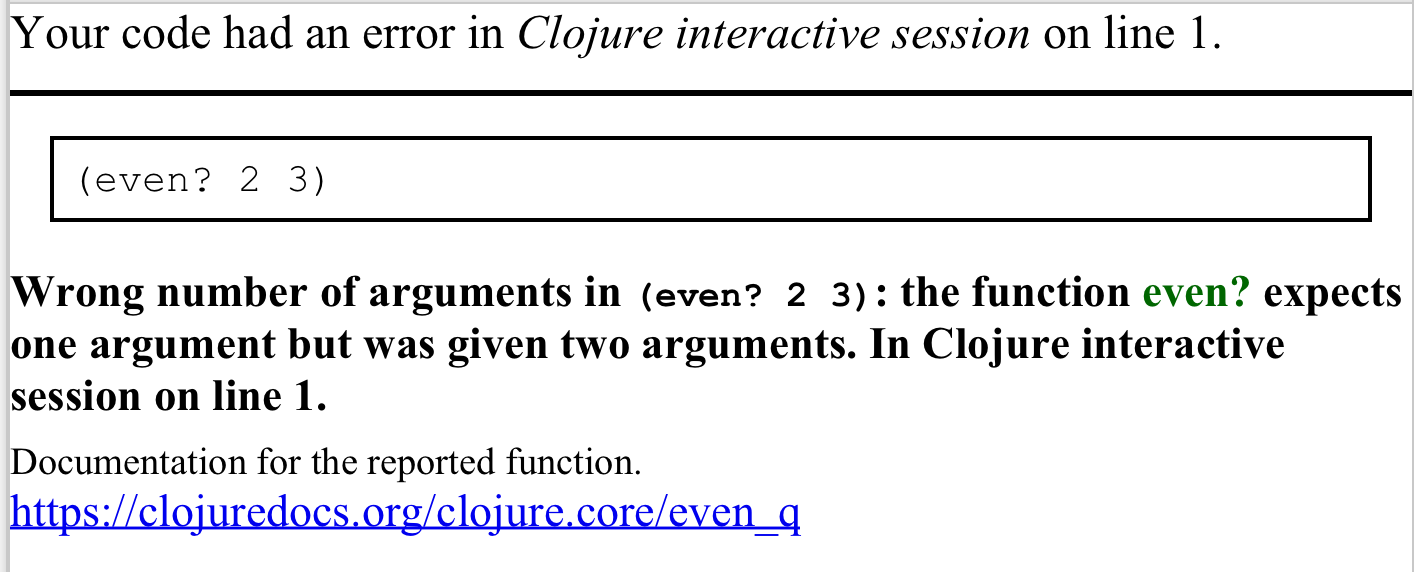
\includegraphics[width=\linewidth]{figures/ErrorViewer2Cropped.png}
}

\column{0.3}
\block{Progress This Year.}{
%\jwcomment{John's section.}
    \begin{itemize}
        \item We improved internal tooling to allow us to easily select different types of error messages and test how they are presented.
        \item We implemented a skeleton framework for data flow to the interactive viewer.
        \item We created a system for labeling parts of an error message to be able to use different formats for different parts.
        \item We created a simple viewer to format error messages based on labeled data.
    \end{itemize}
}

\block{Future Work.}{
%\jscomment{Jaydon's section.}
    \begin{itemize}
        \item We would like to develop more Morse viewers for other information provided in error messages, such as stack traces and Java errors. \emcomment{To allow users open and close different parts of an error message to get as much information as they need?}
        \item We are looking to conduct usability studies on Morse \emcomment{displaying error messages in Morse?} in the future.
        \item We also want to explore integrating Morse viewers into IDEs such as Visual Studio Code for workflow refinements.
        \item We are considering adding support for defining terms in messages via hover text, as well as providing more access to resources like documentation.
    \end{itemize}
}

\block{Acknowledgments}{
 Thanks to Morris Academic Partnership (MAP) and the Undergraduate Research Opportunity (UROP) for funding this work. \\
Thanks to Joe Lane (Nubank) for guidance on tools for this project. 
}

\block{Sources}{
    \begin{itemize}
        \item {[1]} \emph{clojure.org}
        \item {[2]} Morse, Nubank \emph{https://github.com/nubank/morse}
	\item {[3]} Tao Dong, Kandarp Khandwala,  \textit{The Impact of ``Cosmetic'' Changes on the Usability of Error Messages}, 2019 CHI Conference on Human Factors in Computing Systems.
	\item {[4]} Matthias Felleisen, Robert Bruce Findler, Matthew Flatt, and Shriram Krishnamurthi \textit{The Structure and Interpretation of the Computer Science Curriculum},  Journal of Functional Programming, 2004.
    \end{itemize}
}

\block{}{
\begin{tikzfigure}
    
\includegraphics[width=0.5\linewidth]{figures/UMM logo.png}
\end{tikzfigure}
}

\end{columns}


\end{document}
